\chapter{Pendahuluan}
\label{chap:intro}

\section{Latar Belakang}
\label{sec:1:latar_belakang}

Institusi yang memberikan pendidikan, perlu memiliki cara untuk mengetahui pemahaman pelajarnya. Salah satu caranya adalah dengan memberikan tugas. Tugas merupakan sebuah bentuk penilaian dari pengajar kepada pelajarnya~\cite{febriana:plagiarisme}. Tugas diberikan kepada pelajar untuk membantu pelajar mendalami materi yang sudah diberikan sebelumnya oleh pengajar dan juga untuk melihat seberapa jauh pemahaman pelajar terhadap materi yang sudah diberikan.

% TODO: Masukkin referensi di sini ~\cite{onder:judge}
Pada bidang informatika, banyak materi pembelajaran yang dapat diberikan. Salah satu pembelajaran utama dalam bidang informatika adalah keterampilan pemrograman. Dikarenakan itu, perlu sebuah sistem untuk melatih keterampilan pemrograman yaitu dengan memberikan tugas menulis kode program sesuai dengan petunjuk yang diberikan dan program tersebut dapat berjalan sesuai dengan petunjuk\iffalse~\cite{onder:judge}\fi. Secara tradisional, tugas ini diberikan dengan cara pengajar menyiapkan dan mendistribusikan tugas tersebut kepada pelajar, kemudian dikumpulkan kembali hasil program pekerjaan pelajar, dan pengajar akan menilai kode program sesuai ketepatan dengan program yang diinginkan secara manual seperti gambar \ref{fig:1:tradisional}. Karena menilaian kode program mencakup keluaran program dan juga analisis kode, maka proses tersebut memakan waktu yang cukup lama untuk dilakukan. Walaupun begitu, cara tradisional ini masih bekerja jika jumlah pelajarnya sedikit.
Tetapi semakin banyak kode program yang harus di periksa maka semakin banyak waktu yang dibutuhkan dan semakin banyak pula kesalahan yang berhubungan dengan manusia. Salah satu masalah lain yang muncul juga adalah pelajar tidak dapat mengetahui apakah kode program berada pada jalur yang benar dalam menemukan solusi tugas tersebut.

\begin{figure}[H]
    \centering
    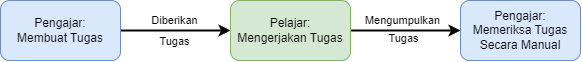
\includegraphics[width=0.8\textwidth]{latar_belakang/tradisional.drawio.png}
    \caption[Sistem Tradisional Pemberian Tugas]{Sistem Tradisional Pemberian Tugas}
    \label{fig:1:tradisional}
\end{figure}

Pemberian tugas menulis kode program memiliki banyak masalah. Oleh karena itu, dibutuhkannya sistem baru untuk memberikan tugas kepada pelajar bidang informatika. Sistem baru yang dimaksud tentunya untuk melakukan penilaian secara otomatis. Sebuah sistem yang mengambil kode program pelajar dan memberikan sebuah nilai numerik yang menandakan hasil dari kode program tersebut~\cite{kurnia:onlinejudge}. Suatu hal yang menarik, Tugas kode program dapat dibagi menjadi 2 jenis yaitu tugas individu dan tugas kelompok. Pada tugas kelompok merupakan tugas yang ditanggung oleh banyak pelajar, biasanya program yang dibuat memiliki antarmuka dan harus diperiksa oleh pengguna khusus yang mengetahui fitur-fitur yang dibutuhkan. Sedangkan tugas individu merupakan sebuah tugas yang diberikan untuk satu individu, biasanya program yang dibuat bersifat algoritmik dan tidak memerlukan antarmuka untuk dijalankan. Program algoritmik sebuah jenis program yang dibuat berdasarkan algoritma untuk menyelesaikan masalah tertentu. Algoritma sendiri adalah langkah-langkah dalam pemecahan masalah secara sistematis~\cite{idcloudhost:algorithm}.
% FIXME: ini kalimat line 16, asa kurang tp buat memperjelas gt 
Algoritma itu seperti resep makanan, dimana akan ada bahan-bahan yang dibutuhkan dan serangkaian langkah untuk membuat suatu makanan yang dijelaskan.

Sebagian besar program yang bersifat algoritmik hanyak perlu mengambil \textit{input} dari \textit{input} standar seperti angka, huruf, dan sebuah kata atau kalimat dengan format yang sudah ditentukan, seolah-olah \textit{input} ini merupakan \textit{output} dari program lain. Kemudian program algoritmik akan memproses \textit{input} tersebut dalam komputer dan mengeluarkan hasil komputasinya dalam format yang sudah ditentukan untuk dibaca oleh program lain dan memanfaatkan hasil komputasi tersebut. Singkatnya, program algoritmik itu seperti filter antar program. Dengan ini, sistem penilaian secara otomatis dapat dibuat dengan membuat sebuah program yang mengambil kode program, memasukkan \textit{input} sesuai format ke dalam program tersebut, membaca hasil keluaran program, dan menilai hasil keluaran program tersebut~\cite{kurnia:onlinejudge}. Sistem penilaian otomatis \mbox{ini diberikan nama \textit{Online Judge}}. Terlebih lagi sistem ini dapat dilakukan secara \textit{offline} maupun \textit{online}. Gambar \ref{fig:1:onlinejudge} menunjukkan bagaimana \textit{online judge} berintegrasi dengan sistem pemberian tugas yang sudah ada.

\begin{figure}[H]
    \centering
    
\includegraphics[width=\textwidth]{latar_belakang/online_judge.drawio.png}
    \caption[Sistem Integrasi oleh \textit{Online Judge}]{Sistem Integrasi oleh \textit{Online Judge}}
    \label{fig:1:onlinejudge}
\end{figure}

Tugas pemrograman sudah menjadi keseharian dalam pembelajaran pada bidang informatika.
Termasuk pada perguruan tinggi pada bidang informatika, maka \textit{online judge} menjadi sebuah kebutuhan termasuk pada Universitas Katolik Parahyangan atau yang biasa disebut UNPAR.
\textit{Online Judge} yang digunakan oleh UNPAR dinamakan SharIF-Judge~\cite{stillmen:sharif} yang merupakan hasil dimodifikasi oleh Stillmen Vallian terhadap Sharif-Judge~\cite{javed:sharif} buatan Mohammad Javad Naderi yang dibuat menggunakan \textit{framework} CodeIgniter dan Bash. Gambar~\ref{fig:1:dashboardpng} merupakan halaman utama setelah masuk ke dalam SharIF-Judge.

\begin{figure}[H]
    \centering
    \includegraphics[width=0.8\textwidth]{views/dashboard.png}
    \caption[Tampilan Awal SharIF Judge]{Tampilan Awal SharIF Judge}
    \label{fig:1:dashboardpng}
\end{figure}

Ujian juga merupakan sebuah bentuk penilaian dari pengajar kepada pelajarnya. Tentunya pelajar maupun mahasiswa ingin memperoleh nilai yang memuaskan dalam ujiannya. Banyak cara yang dilakukan oleh pelajar maupun mahasiswa untuk memperoleh nilai tersebut, salah satunya adalah dengan melakukan kecurangan yaitu \textit{copy paste} atau menyalin jawaban teman atau rekan mereka~\cite{febriana:plagiarisme}. Praktek ini diperparah jika ujian dilakukan secara \textit{online}, dikarenakan pelajar dapat mengakses berbagai fasilitas di internet. Oleh karena itu, diperlukanyna sebuah sistem pada sistem \textit{online judge} untuk mengawasi saat terjadinya ujian online.

Pada saat siswa mengerjakan tugas maupun ujian pembuatan kode program, umumnya pengerjaan kode tersebut dilakukan pada aplikasi eksternal seperti \textit{visual studio code} atau \textit{notepad}. Hal ini juga terjadi pada sistem dalam UNPAR dimana mahasiswa akan membuat kode program pada aplikasi eksternal. Ini membuat pengawasan saat pembuatan kode program lebih sulit untuk dilakukan, terlebih jika ujian dilakukan secara \textit{online}. Maka dari itu, Nicholas Aditya Halim memodifikasi SharIF Judge agar semua sistem pemberian tugas seperti pada gambar \ref{fig:1:onlinejudge} dapat dilakukan dalam sistem yang sama yaitu pada SharIF Judge. Sistem yang bangun oleh Nicholas Aditya Halim adalah ``Implementasi editor kode pada Sharif Judge''~\cite{nicholas:sharif}, dimana SharIF Judge ditambahkan sebuah \textit{Integrated Development Environment} atau yang disebut dengan IDE. IDE merupakan sebuah sistem yang memiliki kemampuan untuk membuat kode dalam editor kode dan menjalankan kode program tersebut. Dengan adanya IDE, seluruh proses pembuatan kode program dapat dilakukan dalam SharIF Judge. Maka dari itu, seluruh proses sistem pemberian tugas dapat dilakukan dalam satu sistem saja, yaitu SharIF Judge.

Walaupun begitu, pada dasarnya IDE tidak dapat mengawasi jika terjadinya praktek \textit{copy paste}. Maka dari itu pada Tugas akhir ini, IDE pada SharIF Judge akan dimodifikasi untuk menangani hal tersebut dengan ditambahkannya fitur untuk merekam semua ketikan atau kejadian dalam editor kode dalam IDE. Lalu ketikan atau kejadian dalam editor dapat di putar kembali seperti rekaman. Fitur ini akan membuat pengawasan terhadap kegiatan kuliah lebih mudah untuk pengawas dan dapat menjadi bukti kecurangan jika dibutuhkan.

\begin{comment}
Ujian merupakan sebuah alat bantu untuk menilai pemahaman pelajar tentang ilmu yang diberikan oleh pengajar. Salah satu ujian yang diberikan kepada pelajar informatika adalah ujian koding yang biasanya dinilai berdasarkan ketepatan algoritma yang dipakai. Tetapi melakukan penilaian untuk setiap kode merupakan sebuah hal yang sulit untuk dilakukan karena dibutuhkannya waktu yang lama. Maka dari itu website \textit{judge} dibuat untuk memudahkan pekerjaan pengajar.

\textit{Judge} merupakan sebuah website yang akan menilai sebuah kode dengan menjalankannya berdasarkan masukkan yang ditentukan dan menyamakan keluaran dari kode dengan keluaran yang sudah ditetapkan oleh pembuat soal dalam kurun waktu yang ditetapkan. Oleh karena itu, kode yang dibuat harus dapat mencakupi waktu yang diberikan dengan mengunakan algoritma yang tepat. Bukan hanya menilai dengan keluaran yang tetap tetapi \textit{judge} juga dapat mengunakan kode yang sudah dibuat oleh pengajar dan membandingkannya dengan keluaran kode yang di kumpulkan.

Sudah banyak perguruan tinggi informatika yang mengunakan website \textit{judge} dalam pemeriksaan kode pelajar termasuk perguruan UNPAR untuk penilai kode dari para mahasiswanya. Judge yang digunakan adalah SharIF-Judge~\cite{sharif} yang dimodifikasi oleh Stillmen Vallian terhadap Sharif-Judge~\cite{stillmen:sharif} buatan Mohammad Javad Naderi dengan \textit{framework} CodeIgniter dan Bash. Gambar~\ref{fig:1:dashboardpng} merupakan halaman utama setelah masuk ke dalam website SharIF-Judge.

\begin{figure}[H]
    \centering
    \includegraphics[scale=0.25]{dashboard}
    \caption[Tampilan Awal SharIF Judge]{Tampilan Awal SharIF Judge}
    \label{fig:1:dashboardpng}
\end{figure}

Tugas akhir ini merupakan sebuah pengembangan lanjutan dari tugas akhir yang bertopik ``Implementasi editor kode pada Sharif Judge''~\cite{nicholas:sharif} oleh Nicholas Aditya Halim. Tugas akhir tersebut menceritakan bahwa SharIF-Judge tidak memiliki kemampuan untuk mengawasi proses pembuatan kode program karena para mahasiswa menggunakan aplikasi eksternal untuk pembuatan kode program tersebut. Sehingga dibuatnya modifikasi terhadap SharIF-Judge untuk menambahkan \textit{Intergrated Development Enviroment} (IDE), sebuah aplikasi untuk mengedit, mengompilasi, dan menjalankan kode program pada SharIF-Judge dengan editor kode bernama Ace~\cite{ace}. Gambar~\ref{fig:1:editor-kode} merupakan tampilan editor kode yang sudah diimplementasikan pada SharIF-Judge.

\begin{figure}
    \centering
    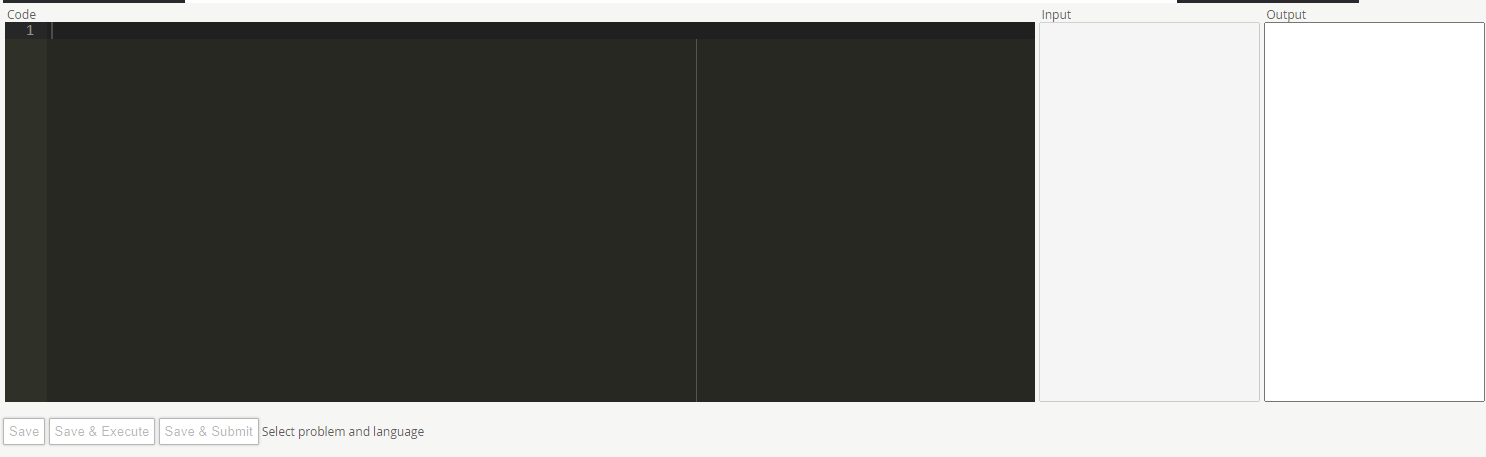
\includegraphics[scale=0.25]{kode-editor}
    \caption[Tampilan editor kode pada SharIF-Judge]{Tampilan editor kode pada SharIF-Judge}
    \label{fig:1:editor-kode}
\end{figure}

Tetapi SharIF Judge masih tidak memiliki kemampuan untuk mengawasi proses pembuatan kode program pada aplikasi eksternal maupun IDE dalam SharIF Judge. Maka dari itu tugas akhir ini menambahkan fitur pada SharIF Judge dengan merekam ketikan pada IDE yang tersedia di SharIF-Judge untuk membantu pengawasan dengan merekam dan memutar ulang ketikan mahasiswa. Tugas akhir ini akan membuat pengawasan terhadap kegiatan kuliah lebih mudah untuk pengawas dan dapat menjadi bukti kecurangan jika dibutuhkan.
\end{comment}

\section{Rumusan Masalah}
\label{sec:1:rumusan}

Rumusan Masalah yang akan dibahas pada tugas akhir ini adalah:
\begin{enumerate}
    % \item Bagaimana agar editor kode lebih mudah untuk dipakai oleh mahasiswa.
    \item Bagaimana mengimplementasikan perekaman dan pemutaran ulang ketikan mahasiswa pada IDE SharIF-Judge?
    \item Bagaimana cara menyimpan data pemutaran ulang mahasiswa secara rutin dengan otomatis dan tidak mengambil penyimpanan \textit{database} sangat besar?
    \item Bagaimana tanggapan pengguna terhadap implementasi perekaman dan pemutaran ulang kode ketikan pada SharIF Judge?
\end{enumerate}

\section{Tujuan}
\label{sec:1:tujuan}

Tujuan yang ingin dicapai skripsi ini adalah sebagai berikut:
\begin{enumerate}
    \item Mengimplementasikan perekaman dan pemutaran ulang ketikan mahasiswa pada IDE SharIF-Judge.
    \item Mencari cara penyimpanan data efektif dan mengimplementasikannya pada perekaman dan pemutaran ulang ketikan.
    \item Mendapatkan umpan balik dari tanggapan pengguna terhadap perekaman dan pemutaran ulang ketikan mahasiswa pada SharIF-Judge.
\end{enumerate}

\section{Batasan Masalah}
\label{sec:1:batasan}

Pada pengerjaan tugas akhir ini terhadap batasan sebagai berikut:
\begin{itemize}
    \item Perangkat lunak SharIF Judge hanya digunakan pada lingkungan Teknik Informatika Unpar.
    \item Perangkat lunak hanya dapat diuji pada mata kuliah pemrograman di mana dosen pembimbing terlibat.
\end{itemize}

\section{Metodologi}
\label{sec:1:metlit}

Metodologi pengerjaan tugas akhir ini adalah sebagai berikut:
\begin{enumerate}
    \item Melakukan studi mengenai komponen yang diperlukan untuk membuat sistem perekaman dan pemutaran ulang ketikan pada IDE berbasis web.
    \item Merancang sistem perekaman dan pemutaran ulang ketikan berbasis web untuk SharIF Judge
    \item Mengimplementasikan IDE berbasis web pada SharIF Judge.
    \item Melakukan pengujian dan eksperimen.
    \item Menulis dokumen tugas akhir.
\end{enumerate}

\section{Sistematika Pembahasan}
\label{sec:1:sispem}

Sistematika pembahasan skripsi ini adalah sebagai berikut:
\begin{itemize}
    \item \textbf{Bab \ref{chap:intro}:} Pendahuluan \\
          Membahas latar belakang, rumusan masalah, tujuan, batasan masalah, metodologi, dan sistematika pembahasan.
    \item \textbf{Bab \ref{chap:teori}:} Landasan Teori \\
          Membahas teori-teori yang berhubungan dengan penelitian ini, yaitu SharIF Judge, CodeIgniter 3, Twig, IDE, dan Ace.
    \item \textbf{Bab 3:} Analisis \\
          Membahas analisis terhadap perangkat lunak SharIF Judge dan IDE pada SharIF Judge.
    \item \textbf{Bab 4:} Perancangan \\
          Membahas perancangan fitur yang diimplementasikan pada SharIF Judge.
    \item \textbf{Bab 5:} Implementasi dan Pengujian \\
          Membahas implementasi fitur pada SharIF Judge dan pengjuan yang dilakukan.
    \item \textbf{Bab 6:} Kesimpulan dan Saran \\
          Membahas kesimpulan dari penelitian ini dan saran untuk penelitian berikutnya.
\end{itemize}